%______________________________________________________________________
\documentclass[xcolor=dvipsnames]{beamer}
%\usetheme{default}
%______________________________________________________________________
\usepackage[T1]{fontenc}
\usepackage[ansinew]{inputenc}
%\usepackage[latin1]{inputenc}
\usepackage[spanish]{babel}
\usepackage{amsmath,amssymb,amsthm}
\usepackage{graphicx,graphics}
\usepackage{amsmath, amsthm, amssymb, amsfonts}
\usepackage{enumerate}
\usepackage{multicol}
\usepackage{url}     
\usepackage{hyperref}
%______________________________________________________________________
\title{Un primer estudio no cualitativo de la certificaci\'on en la UACM} 
\author{Carlos E Mart\'inez-R\\
.\\
\tiny{La certificaci\'on como un problema de modelaci\'on
matem\'atica y datos grandes}\\
.\\
\tiny{\textit{Encuentro de experiencias de revisi\'on de planes y programas de estudios}}
}
%______________________________________________________________________
\pgfdeclareimage[height=0.7cm]{logo-izq}{logouacm.png}
\pgfdeclareimage[height=0.7cm]{logo-der}{mascotauacm.jpg}
\logo{\pgfuseimage{logo-der}} \setbeamertemplate{sidebar left}
{\logo{\pgfuseimage{logo-izq}}
\vfill %pone la imgen en la esquina inferior izquierda
\rlap{\hskip0.1cm\insertlogo} %inserta la imgen
\vskip15pt}
%______________________________________________________________________
\useoutertheme{infolines}
\usetheme{Ilmenau}% esta bueno cal=7
%\usetheme{Warsaw} % me gusta cal=7
%\usetheme{Malmoe} %muy simple
%\usetheme{boxes}% muy chafa! cal=5
%\usetheme{Rochester} % me gusta!, calificación = 6, pues le faltan los pies de página.
%\usetheme{Szeged} %No me gusta
%\usetheme{AnnArbor} % demasiado colorida
%\usetheme{Copenhagen} % parecida a una anterior, es decir, pelas!
%\usetheme{Dresden} % leve, cal=5
%\usetheme{Pittsburgh} %chafa!!!
%\usetheme{Luebeck}
%\usetheme{Berkeley}
%___________________________________________________________________________________________________________________
%
\begin{document}
\setbeamertemplate{navigation symbols}{}
%_____________________________________________________________________________________%1
\begin{frame}
%\makeindex
  \maketitle

\end{frame}


\section*{}
\small
\begin{frame}
\tableofcontents
\end{frame}
%


%\begin{frame}
\section{La Universidad Aut\'onoma de la Ciudad de M\'exico}


\begin{frame}\frametitle{Introducci\'on y antecedentes}



\subsection{Introducci\'on y antecedentes}

\begin{itemize}

\item La Universidad Aut\'onoma de la Ciudad de M\'exico fue creada el 26 de abril de 2001 por el gobierno del Distrito federal a trav\'es del \href{https://www.uacm.edu.mx/Portals/0/adam/Content/hfXbhKHHXE2k2Y8j2fG9UQ/Text/DCUACM.pdf}{decreto de creaci\'on} publicado en la Gaceta Oficial del Distrito Federal por el Jefe de gobierno de la Ciudad de M\'exico, m\'as adelante, 

\item el 16 de diciembre de 2004 la Asamblea Legislativa del Distrito Federal, III Legislatura, aprob\'o la \href{https://www.uacm.edu.mx/Portals/0/ley_uacm092011.pdf}{Ley de la Universidad Aut\'onoma de la Ciudad de M\'exico} misma que fue publicada el 5 de enero de 2005.

\end{itemize}
\end{frame}


\begin{frame}\frametitle{Introducci\'on y antecedentes}

\begin{itemize}

\item El \href{https://drive.google.com/file/d/0B6AEksrqo4h1M2Q5OWVhOGEtODNlNy00M2M2LThkNTctZjE0ZjA4ZGJlZWZj/view?resourcekey=0-9eA5mzOWlPqKF8MTeYH9Iw}{proyecto educativo de la UACM} enuncia que una de las acciones educativas en funci\'on del aprendizaje del estudiante, es procurar que los planes de estudio permitan trayectorias flexibles y que los programas de estudio sean en todo coherentes con sus prop\'ositos formativos, que las formas de evaluaci\'on y presentaci\'on de resultados sean \'utiles a las y los estudiantes, aportando orientaciones  para superar sus dificultades y permitir avanzar en el logro de sus metas de formaci\'on universitaria.

\end{itemize}

\end{frame}


\begin{frame}\frametitle{Introducci\'on y antecedentes}
\begin{itemize}

\item \textit{En la UACM la evaluaci\'on para certificaci\'on tiene la finalidad de dar fe de que el estudiante posee los conocimientos que el certificado ampara. En este sentido se trata de un procedimiento con car\'acter jur\'adico-administrativo, separado de los procesos de ense\~nanza y aprendizaje y las evaluaciones formativas que les son inherentes} \cite{ProyectoEducativo}, 

\item Separar los procesos de ense\~nanza y aprendizaje del de certificaci\'on permite que las y los estudiantes centren su atenci\'on en aprender,  valorando sus propios procesos as\'i como los conocimientos construidos sin la presi\'on de un \'unico momento para certificarlos. 

\item Lo anterior permite que las y los estudiantes se puedan registrar y presentarse en cualquiera de las materias que cubre la oferta acad\'emica sin importar d\'onde, o c\'omo los obtuvieron. 



\end{itemize}
\end{frame}


\begin{frame}\frametitle{Introducci\'on y antecedentes}
\begin{itemize}

\item El \'area responsable de coordinar y realizar los procesos de evaluaci\'on de conocimientos con fines de certificaci\'on, ya sea para materias espec\'ificos, ciclos e incluso de titulaci\'on es la Coordinaci\'on de Certificaci\'on y registro \cite{ProyectoEducativo}.

\item Formalmente la certificaci\'on se define como el proceso mediante el cual la Universidad Aut\'onoma de la Ciudad de M\'exico eval\'ua los conocimientos y competencia con que cuenta el y la estudiante \cite{CircularCertificacion}.


\item La certificaci\'on es aplicada por comit\'es de certificaci\'on, grupo colegiado integrado por profesores investigadores y profesoras investigadoras  nombradas por las academias,  conforme lo establece la circular para regular los procesos y procedimientos de certificaci\'on \cite{CircularCertificacion}.


\end{itemize}

\end{frame}


\begin{frame}\frametitle{Introducci\'on y antecedentes}
\begin{itemize}

\item Modalidades de certificaci\'on: elaboraci\'on de un portafolio,  proyectos, carpetas de trabajo,  presentaci\'on de un \'unico examen de evaluaci\'on de contenidos conforme al programa de estudios.



\item 
\textbf{Las y los estudiantes pueden presentarse cuantas veces lo consideren necesario, las pruebas se basan en el programa del curso \cite{Doc3}}.

\item Desde su creaci\'on la Universidad ha ofertado hasta 1332 distintas materias , algunas de ellas han cambiado su nombre, algunas otras a traves de la modificaci\'on del programa de estudio se han dividido en dos materias.

\end{itemize}

\end{frame}


\section{Metodolog\'ia}

\subsection{Preprocesamiento de datos}

\begin{frame}\frametitle{Preprocesamiento de datos}
\begin{itemize}

\item La informaci\'on se encontraba concentrada en dos archivos con m\'as de un mill\'on de entradas con 10 columnas en un archivo y m\'as de doscientos mil entradas en otro archivo con la misma cantidad de columnas, en las cuales se inclu\'ia la generaci\'on a la que pertenece el estudiantes, su matr\'icula, el nombre de la carrera en curso,  plantel de adscripci\'on, turno, situaci\'on (suspensi\'on tempora, titulado,   activo,  egresado,  baja definitiva o baja temporal), materia, tema espec\'ifico, calificaci\'on y periodo de certificaci\'on.


\end{itemize}

\end{frame}


\begin{frame}\frametitle{Preprocesamiento de datos}
\begin{itemize}

\item Los datos considerados son desde la generaci\'on 1 hasta la generaci\'on 21, es decir, todas aquellas personas estudiantes que se han inscrito en la Universidad para cualquiera de las licenciaturas que se ofrecen: \textit{Ingenier\'ia en Sistemas Electr\'onicos y de Telecomunicaciones, Arte y Patrimonio Cultural, Ciencia Pol\'itica y Administraci\'on Urbana, Ciencias Ambientales y Cambio Clim\'atico, Ciencias Gen\'omicas, Ciencias Sociales, Comunicaci\'on y Cultura, Creaci\'on Literaria, Derecho, Filosof\'ia e Historia de las Ideas, Historia y Sociedad Contempor\'anea, Ingenier\'ia de Software, Ingenier\'ia en Sistemas de Transporte Urbano, Ingenier\'ia en Sistemas Electr\'onicos Industriales, Ingenier\'ia en Sistemas Energ\'eticos, Modelaci\'on Matem\'atica, Nutrici\'on y Salud, Promoci\'on de la Salud y  Protecci\'on Civil y Gesti\'on de Riesgos.}

\end{itemize}




\end{frame}


\begin{frame}\frametitle{Preprocesamiento de datos}
\begin{itemize}

\item Dada la cantidad de informaci\'on y ante la necesidad de unificar ambas bases de datos, se opt\'o por trabajar en \textit{R}, lo cual permiti\'o codificar y procesar las variables y datos a estudiar.


\item 
Una vez unificadas ambas bases de datos se realizaron las siguientes acciones:
para la variable Planteles, se consideraron los cinco planteles en los que se imparten cursos  (\textit{Centro Hist\'orico, Cuautepec, Del Valle, Iztapalapa, San Lorenzo Tezonco}).

\end{itemize}




\end{frame}


\begin{frame}\frametitle{Preprocesamiento de datos}
\begin{itemize}

\item  y todos los dem\'as (\textit{Reclusorio Preventivo Varonil Norte, Centro Escolar Dr. Pedro L\'opez Penitenciar\'ia del Distrito Federal, Centro Escolar Francisco I Madero Centro Femenil de Readaptaci\'on Social de Tepepan, Centro Escolar Francisco I Madero Ceresova Centro de Readaptaci\'on Social Varonil Oriente, Centro Escolar Jos\'e Vasconcelos Ceresova Centro de Readaptaci\'on Social Varonil Sur, Centro Escolar Rosario Ibarra de Piedra Cefereso Centro Femenil de Readaptaci\'on Social Santa Martha Acatitla, Centro Escolar Santiago Ram\'irez, Centro Escolar Valent\'in Campa Salazar Ceresova Centro de Readaptaci\'on Social Varonil Santa Martha Acatitla}) se concentraron en una sola variable: \textit{PESCER}.



\end{itemize}


\end{frame}


\begin{frame}\frametitle{Preprocesamiento de datos}
\begin{itemize}

\item El tratamiento para la variable \textit{Materia} fue un poco m\'as laborioso, con la finalidad de tener \'unicamente texto plano se eliminaron acentos, las min\'usculas se convirtieron en may\'usculas, se eliminaron comilllas, comas y diagonales, se eliminaron las \~ns y di\'eresis. Una vez terminado el preprocesamiento, se ordenaron para contar el n\'umero efectivo de materias registradas en el sistema.



\end{itemize}



\end{frame}


\begin{frame}\frametitle{Preprocesamiento de datos}
\begin{itemize}

\item En lo que corresponde a la variable Tema \textit{Espec\'ifico} al igual que la anterior se eliminaron acentos, di\'eresis, \~ns, diagnoales, se convirti\'o todo a may\'usculas, y finalmente, aquellos valores ausentes se cubrieron por su respectivo valor en la variable \textit{Materia}, es decir, la variable \textit{Tema Espec\'ifico} incluye todos los nombres de las materias junto con los nombres de los seminarios o materias optativas ofertadas en alg\'un momento.
 

\end{itemize}
\end{frame}


\begin{frame}\frametitle{Certificaci\'on en la Universidad}
\begin{itemize}

\item Para la variable \textit{Periodo de Certificaci\'on} su tratamiento fue diferente, primero se proceso cada uno de los datos para que el programa lo pudiera leer efectivamente como fecha, una vez logrado lo anterior, se codific\'o en dos valores: primer y segundo, haciendo referencia al periodo de certificaci\'on correspondiente al primer o segundo semestre del a\~no, uniformizando los distintos valores que estaban registrados de origen. 

\item El procesamiento anterior permiti\'o incorporar una nueva variable relacionada con la certificaci\'on: \textit{a\~no}, misma que se agreg\'o al final de la base de datos.


\item Es en esta parte del proceso en que se puede considerar que termina el preprocesamiento de datos, para dar pie a la revisi\'on y procesamiento de los datos para obtener de cada materia informaci\'on  relacionada con la certificaci\'on
\end{itemize}

\end{frame}


\begin{frame}\frametitle{Preprocesamiento de datos}
\begin{itemize}

\item Es en esta parte del proceso en que se puede considerar que termina el preprocesamiento de datos, para dar pie a la revisi\'on y procesamiento de los datos para obtener de cada materia informaci\'on  relacionada con la certificaci\'on
\end{itemize}

\end{frame}

\subsection{Procesamiento de datos}

\begin{frame}\frametitle{Procesamiento de datos}
\begin{itemize}

\item Cada rengl\'on de la base de datos corresponde a una \textit{matr\'icula} y su respectivo intento (fallido/efectivo) de certificaci\'on para una materia, es decir, puede ocurrir que los primeros 3 renglones correspondan a la misma matr\'icula, misma materia pero distinta calificaci\'on (certificada o no certificada) y distinto periodo de certificaci\'on y distinto a\~no, con lo cu\'al es posible determinar el n\'umero de intentos requeridos para certificar la materia, en caso de que lo haya logrado, cuantos intentos de certificaci\'on realiz\'on sin \'exito, es decir, sin haber logrado certificar la materia; 

\item Tambien es posible determinar si pudo certificar en su primer intento. 


\end{itemize}
\end{frame}


\begin{frame}\frametitle{Procesamiento de datos}
\begin{itemize}

\item Esto se hace para cada estudiante y para cada materia registrada en su historial acad\'emico. 

\item En esta primera aproximaci\'on se decidi\'o que era de inter\'es conocer para cada materia cuales eran las probabilidades de certificar al primer intento, cu\'al es la probabilidad de no certificar nunca la materia, as\'i como informaci\'on  relacionada con los intentos necesarios para certificar la materia.

\item Para el caso de no certificar nunca, se calcularon las tres medidas de tendencia central, as\'i como el valor m\'aximo para los intentos fallidos realizados por certificar la materia.

\end{itemize}

\end{frame}


\begin{frame}\frametitle{Procesamiento de datos}
\begin{itemize}

\item Para el caso de materia s\'i certificada, de manera an\'aloga se calcularon las medidas de tendencia central y el n\'umero m\'aximo de intentos realizados para poder certificar la materia en su \'ultimo intento. 

\item Adem\'as de lo anterior, para cada materia se extrajeron y almacenaron subbases de datos con toda la informaci\'on sin procesar para la materia en turno, un archivo con una tabla de conteo de la informaci\'on correspondiente a la no certificaci\'on, an\'alaogamente para el caso de s\'i certificaci\'on pero no en el primer intento. 

\end{itemize}
\end{frame}

\section{Resultados}

\subsection{Gr\'aficas}

\begin{frame}\frametitle{Certificaci\'on en la Universidad}
\textbf{
\centering{
Cuantas certificaciones se han presentado desde 2001 hasta 2021?
}}
\begin{figure}[H]
\centering
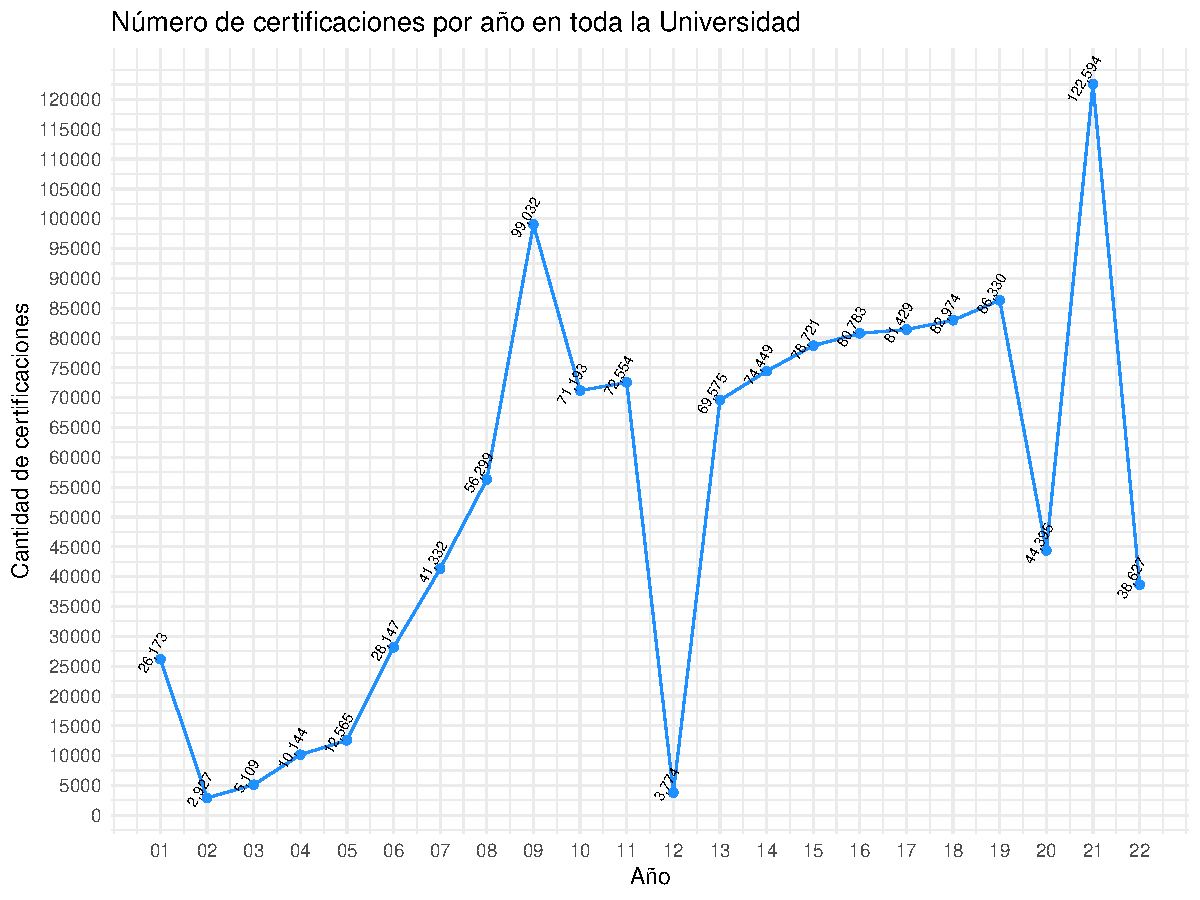
\includegraphics[width=10cm,height=5.5cm]{Imagenes/graficoCertificacionesUACManual.pdf}
\end{figure}
\end{frame}

\begin{frame}\frametitle{Certificaci\'on en planteles (a\~nos) }
\begin{figure}[H]
\centering
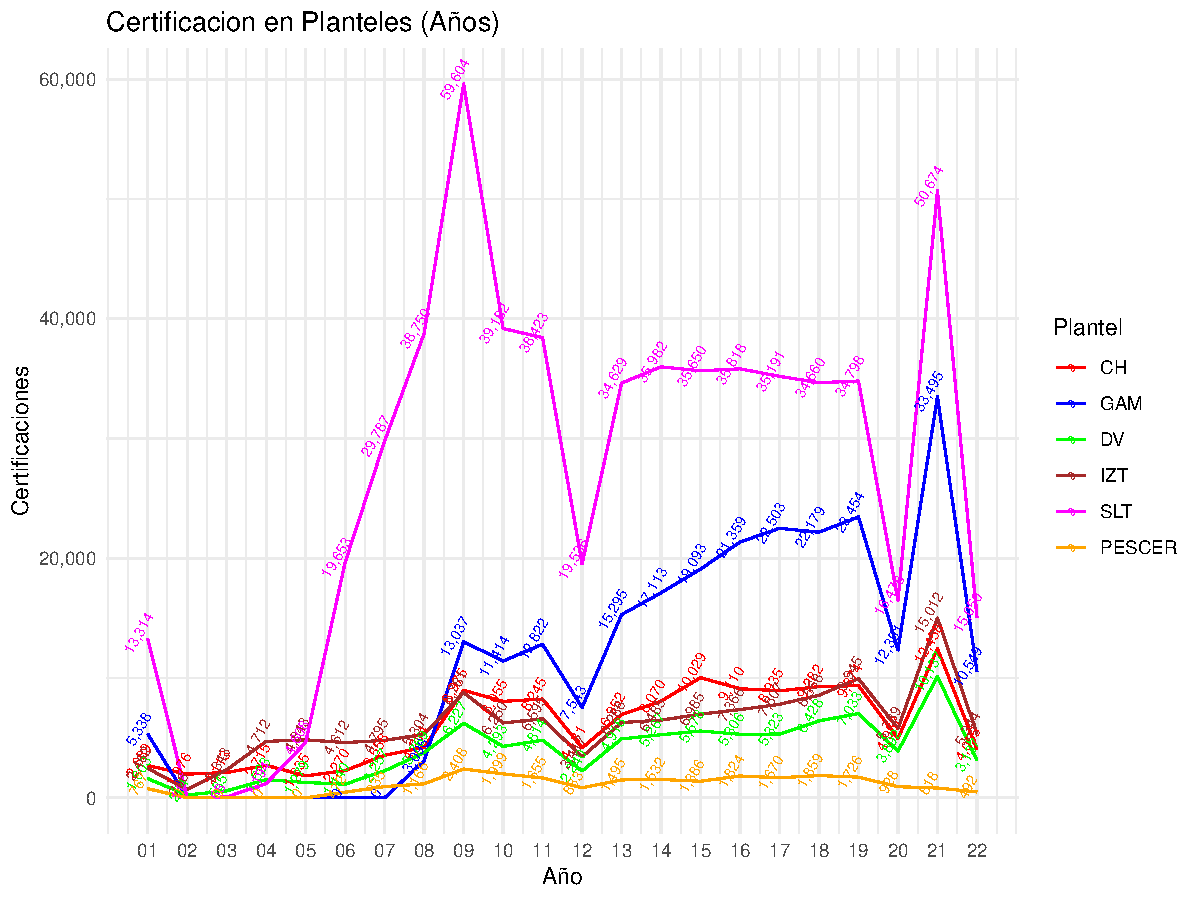
\includegraphics[width=10cm,height=5.5cm]{Imagenes/graficoCertificacionPlantelesAnhos.pdf}
\end{figure}
\end{frame}

\begin{frame}\frametitle{Certificaci\'on en planteles (generaciones)}
\begin{figure}[H]
\centering
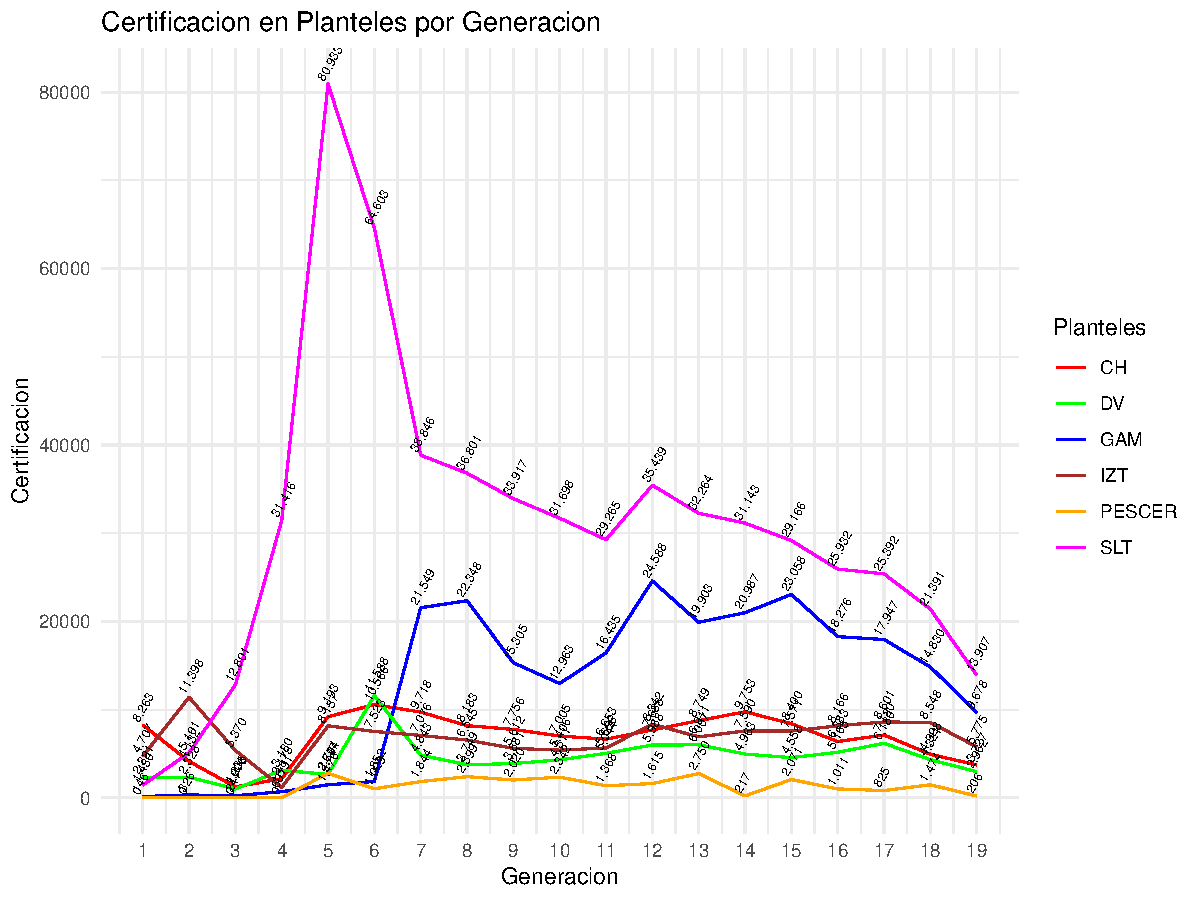
\includegraphics[width=10cm,height=5.5cm]{Imagenes/graficoCertificacionPlantelGeneracion.pdf}
\end{figure}
\end{frame}

\begin{frame}\frametitle{Certificaci\'on (totales) por planteles}
\begin{figure}[H]
\centering
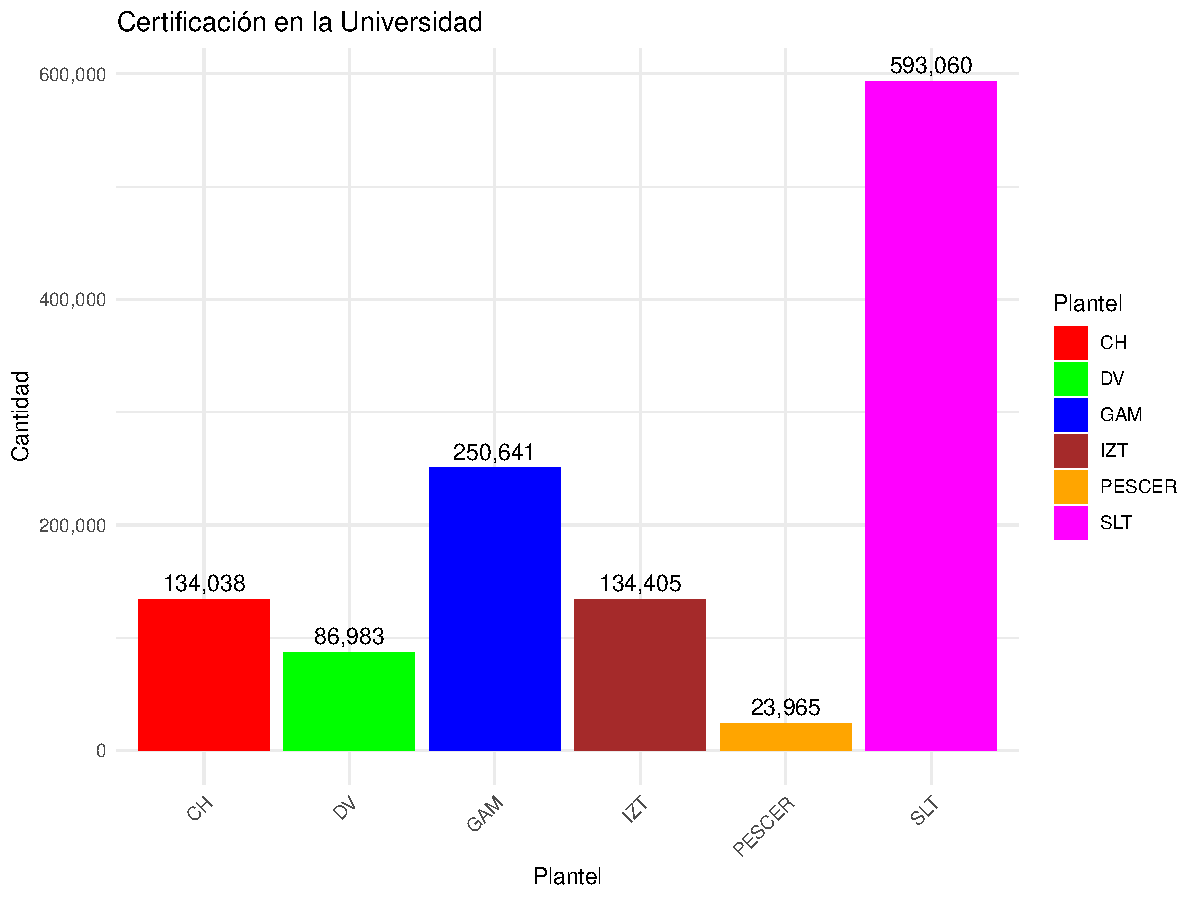
\includegraphics[width=10cm,height=5.5cm]{Imagenes/graficoCertificacionesPlanteles.pdf}
\end{figure}
\end{frame}


\begin{frame}\frametitle{Certificaci\'on (porcentajes) por planteles}
\begin{figure}[H]
\centering
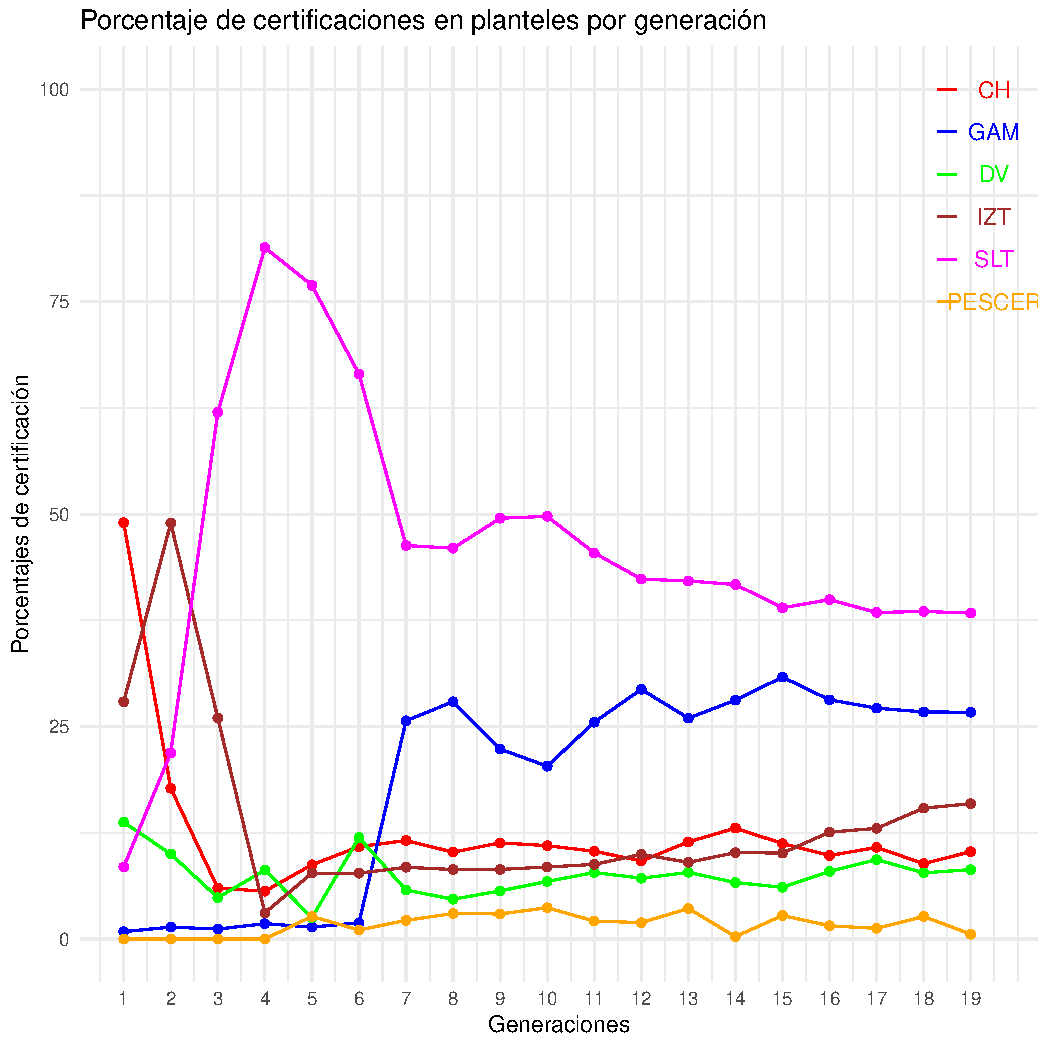
\includegraphics[width=10cm,height=5.5cm]{Imagenes/graficoPorcentajesPlantel.pdf}
\end{figure}
\end{frame}

\begin{frame}\frametitle{Certificaci\'on (totales) en planteles}
\begin{figure}[H]
\centering
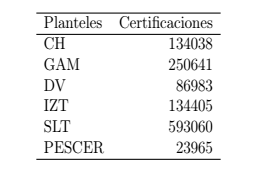
\includegraphics[width=10cm,height=5.5cm]{Tablas/CertificacionPlanteles.png}
\end{figure}
\end{frame}

\begin{frame}\frametitle{Certificaci\'on en planteles (Favorables vs No Favorables)}
\begin{figure}[H]
\centering
\includegraphics[width=10cm,height=5.5cm]{Imagenes/graficoCertificacionPlantelesFnF.pdf}
\end{figure}
\end{frame}

\begin{frame}\frametitle{Certificaci\'on Favorables vs No Favorables en planteles}
\begin{figure}[H]
\centering
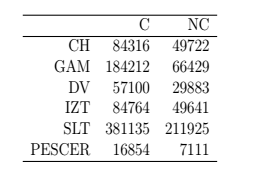
\includegraphics[width=10cm,height=5.5cm]{Tablas/CertificacionFnFPlanteles.png}
\end{figure}
\end{frame}

\begin{frame}\frametitle{Certificaci\'on por licenciaturas}
\begin{figure}[H]
\centering
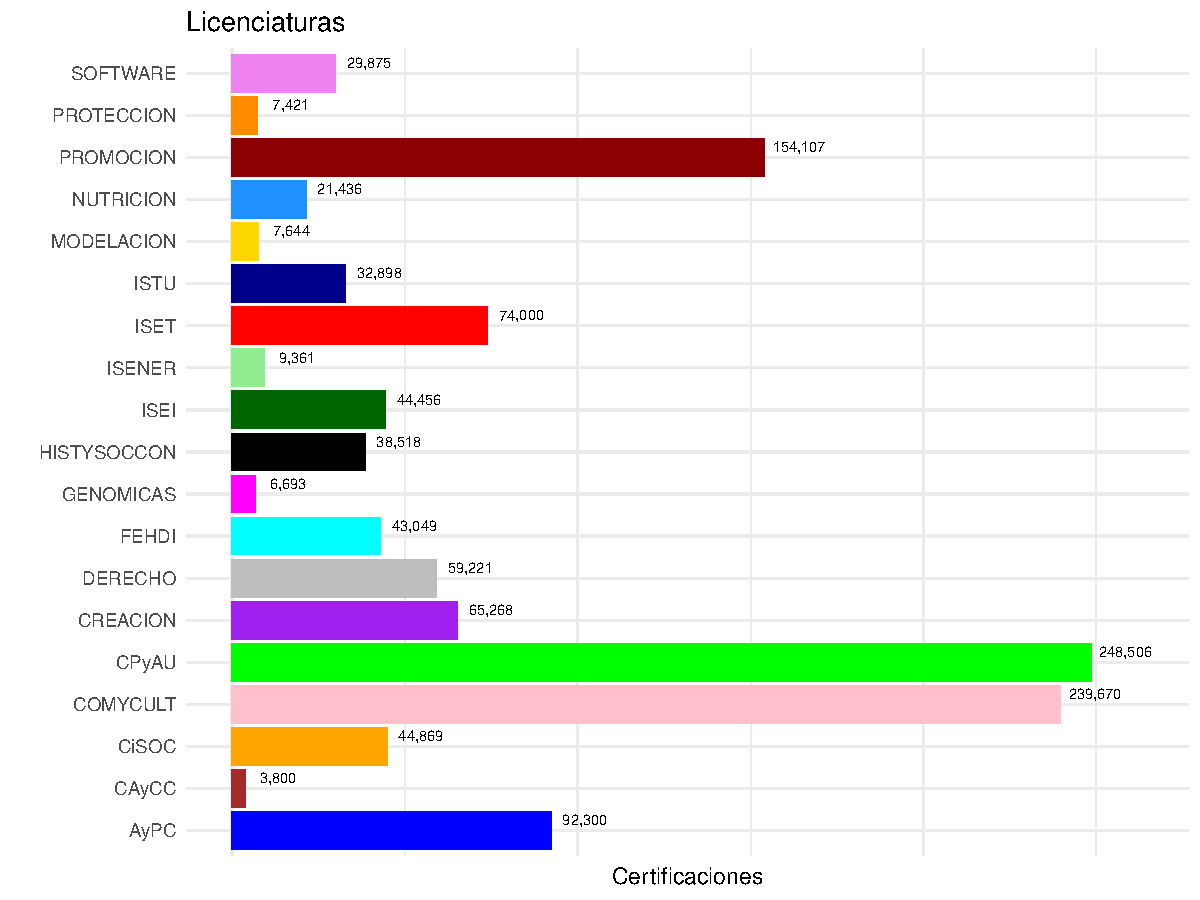
\includegraphics[width=10cm,height=5.5cm]{Imagenes/graficoCertificacionesLicenciaturas.pdf}
\end{figure}
\end{frame}

\begin{frame}\frametitle{Certificaci\'on (totales) licenciaturas}
\begin{figure}[H]
\centering
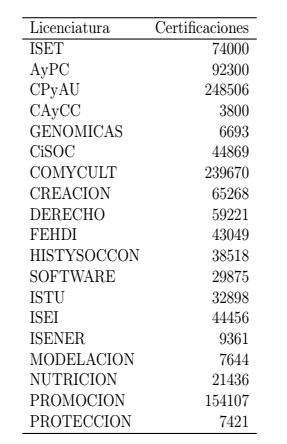
\includegraphics[width=10cm,height=5.5cm]{Tablas/CertificacionTtlLic.png}
\end{figure}
\end{frame}

\begin{frame}\frametitle{Certificaci\'on por licenciaturas}
\begin{figure}[H]
\centering
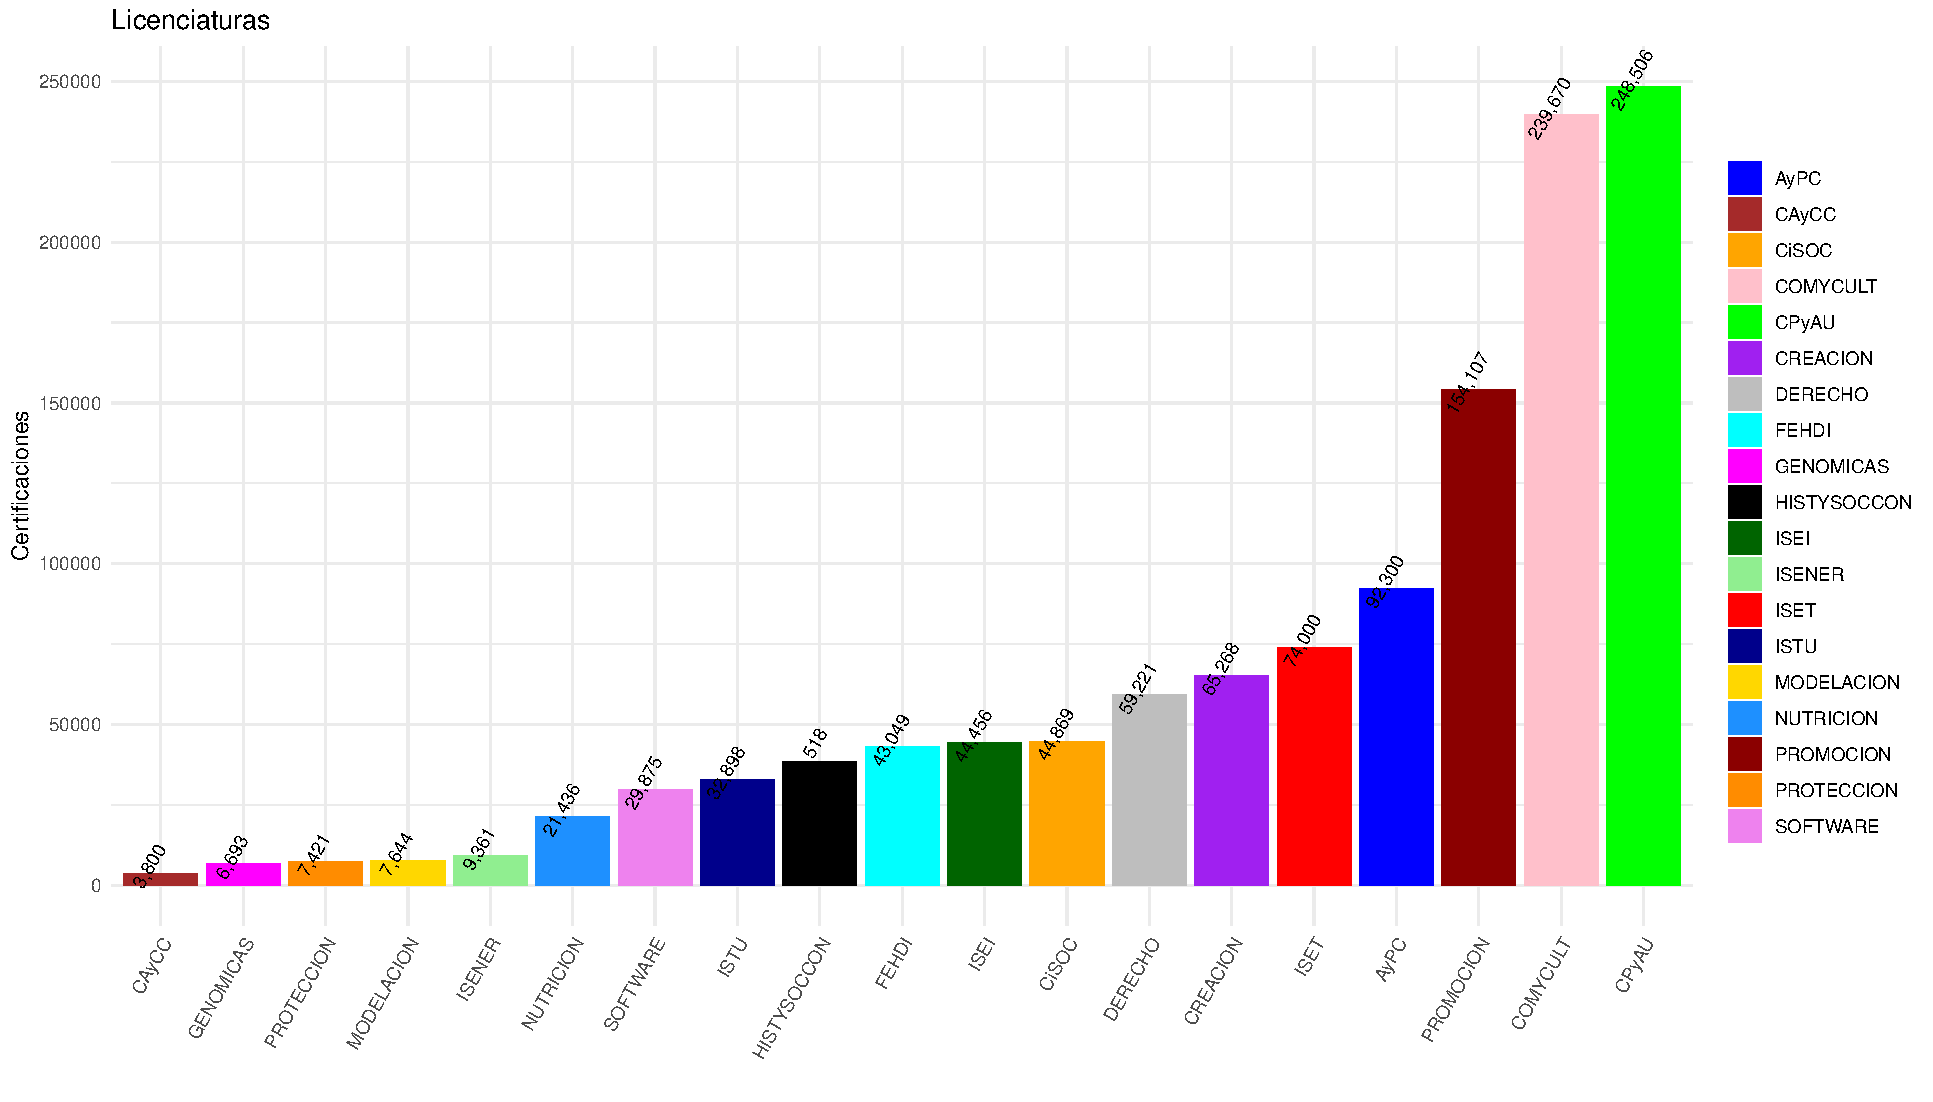
\includegraphics[width=10cm,height=5.5cm]{Imagenes/graficoCertificacionesLicGral.pdf}
\end{figure}
\end{frame}

\begin{frame}\frametitle{Certificaci\'on por licenciaturas en planteles CCyT}
\begin{figure}[H]
\centering
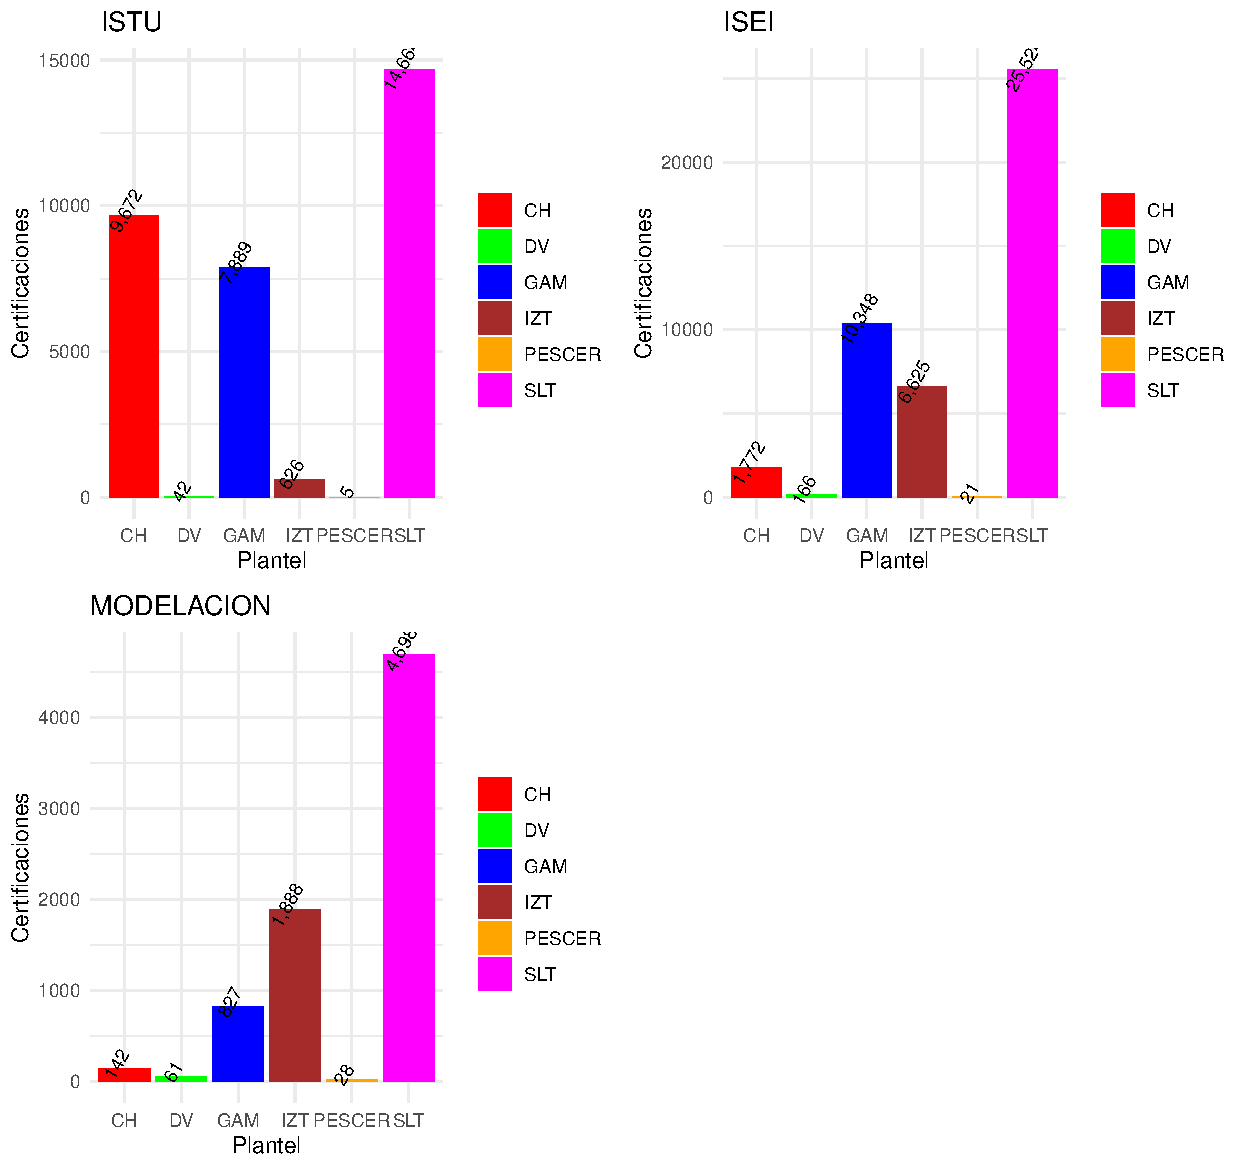
\includegraphics[width=10cm,height=5.5cm]{Imagenes/GraficasCertificacionLicenciaturas1.pdf}
\end{figure}
\end{frame}

\begin{frame}\frametitle{Certificaci\'on por licenciaturas en planteles CCyT}
\begin{figure}[H]
\centering
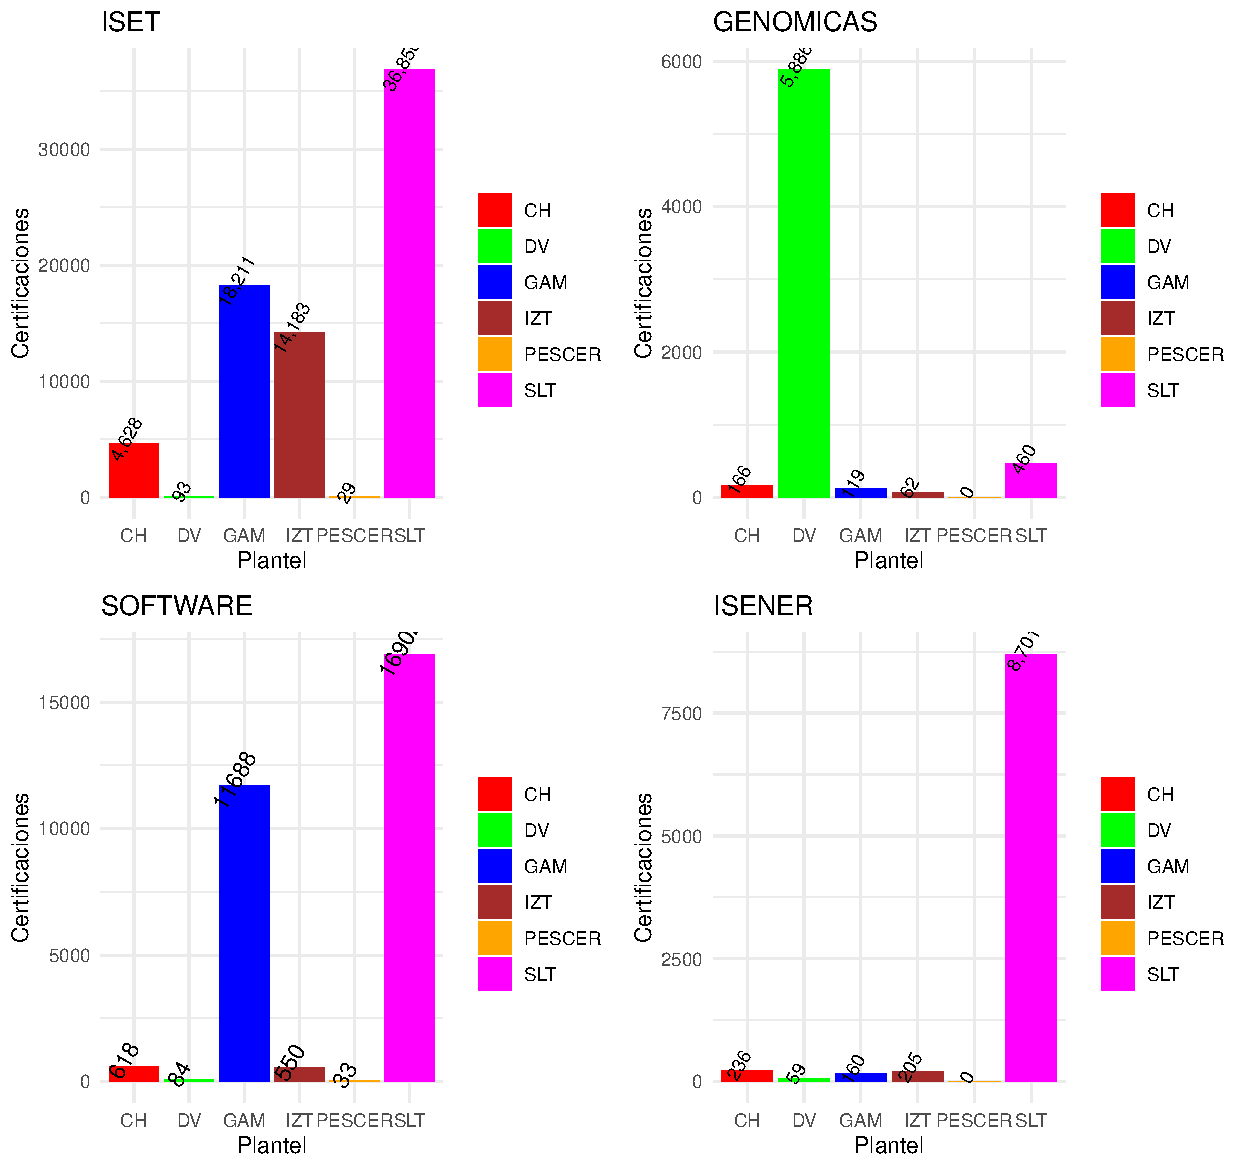
\includegraphics[width=10cm,height=5.5cm]{Imagenes/GraficasCertificacionLicenciaturas2.pdf}
\end{figure}
\end{frame}

\begin{frame}\frametitle{Certificaci\'on por licenciaturas en planteles CCyH}
\begin{figure}[H]
\centering
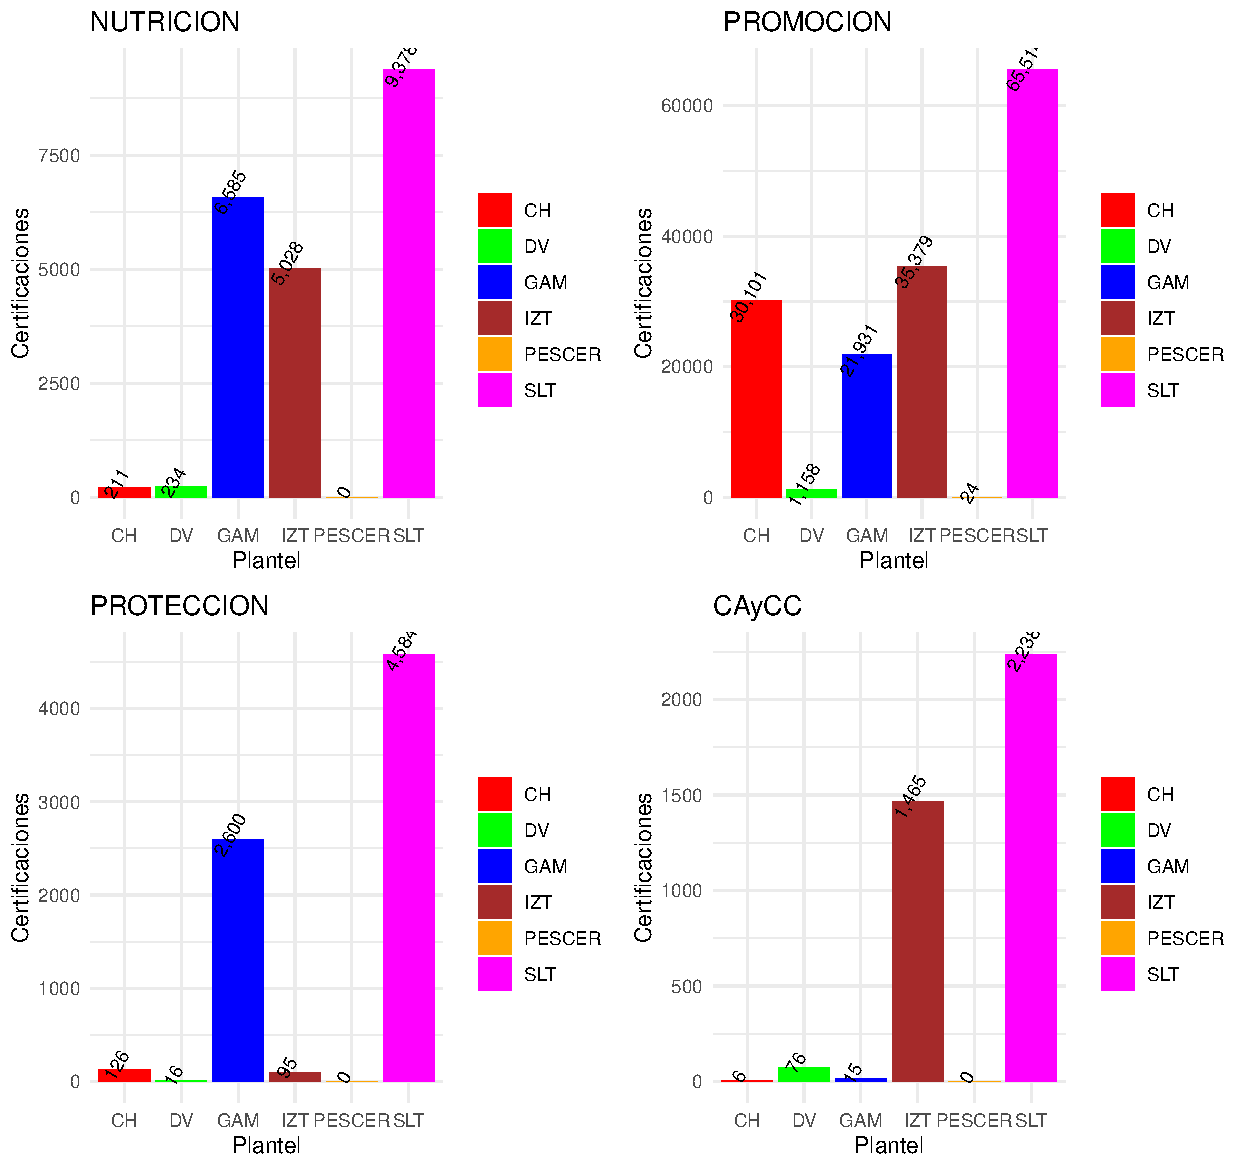
\includegraphics[width=10cm,height=5.5cm]{Imagenes/GraficasCertificacionLicenciaturas3.pdf}
\end{figure}
\end{frame}

\begin{frame}\frametitle{Certificaci\'on por licenciaturas en planteles CHyCS}
\begin{figure}[H]
\centering
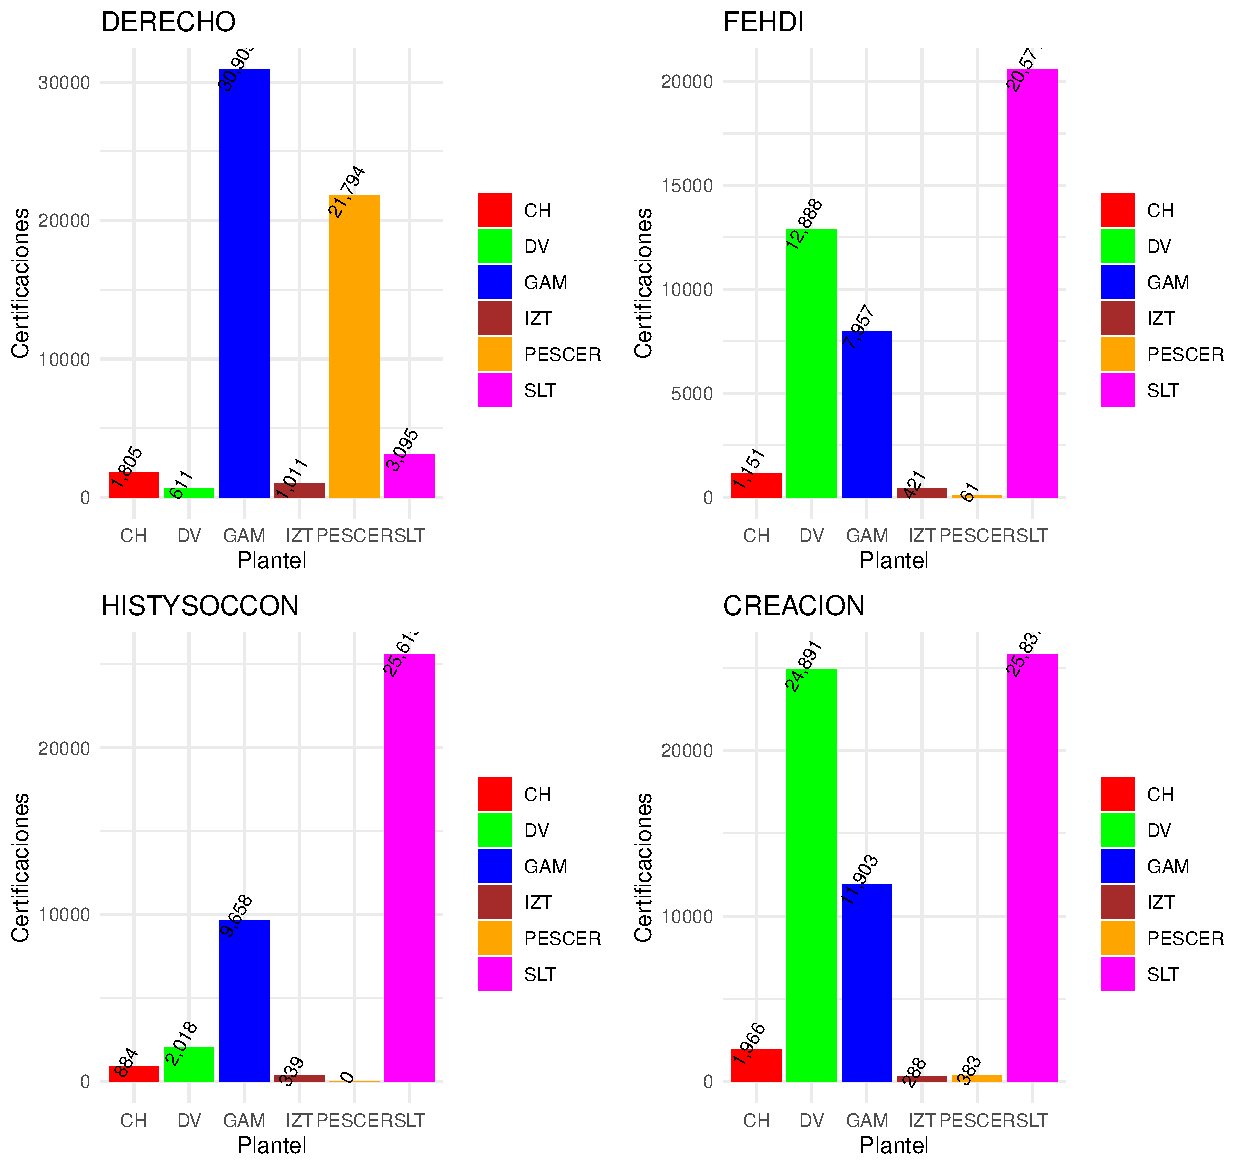
\includegraphics[width=10cm,height=5.5cm]{Imagenes/GraficasCertificacionLicenciaturas4.pdf}
\end{figure}
\end{frame}

\begin{frame}\frametitle{Certificaci\'on por licenciaturas en planteles CHyCS}
\begin{figure}[H]
\centering
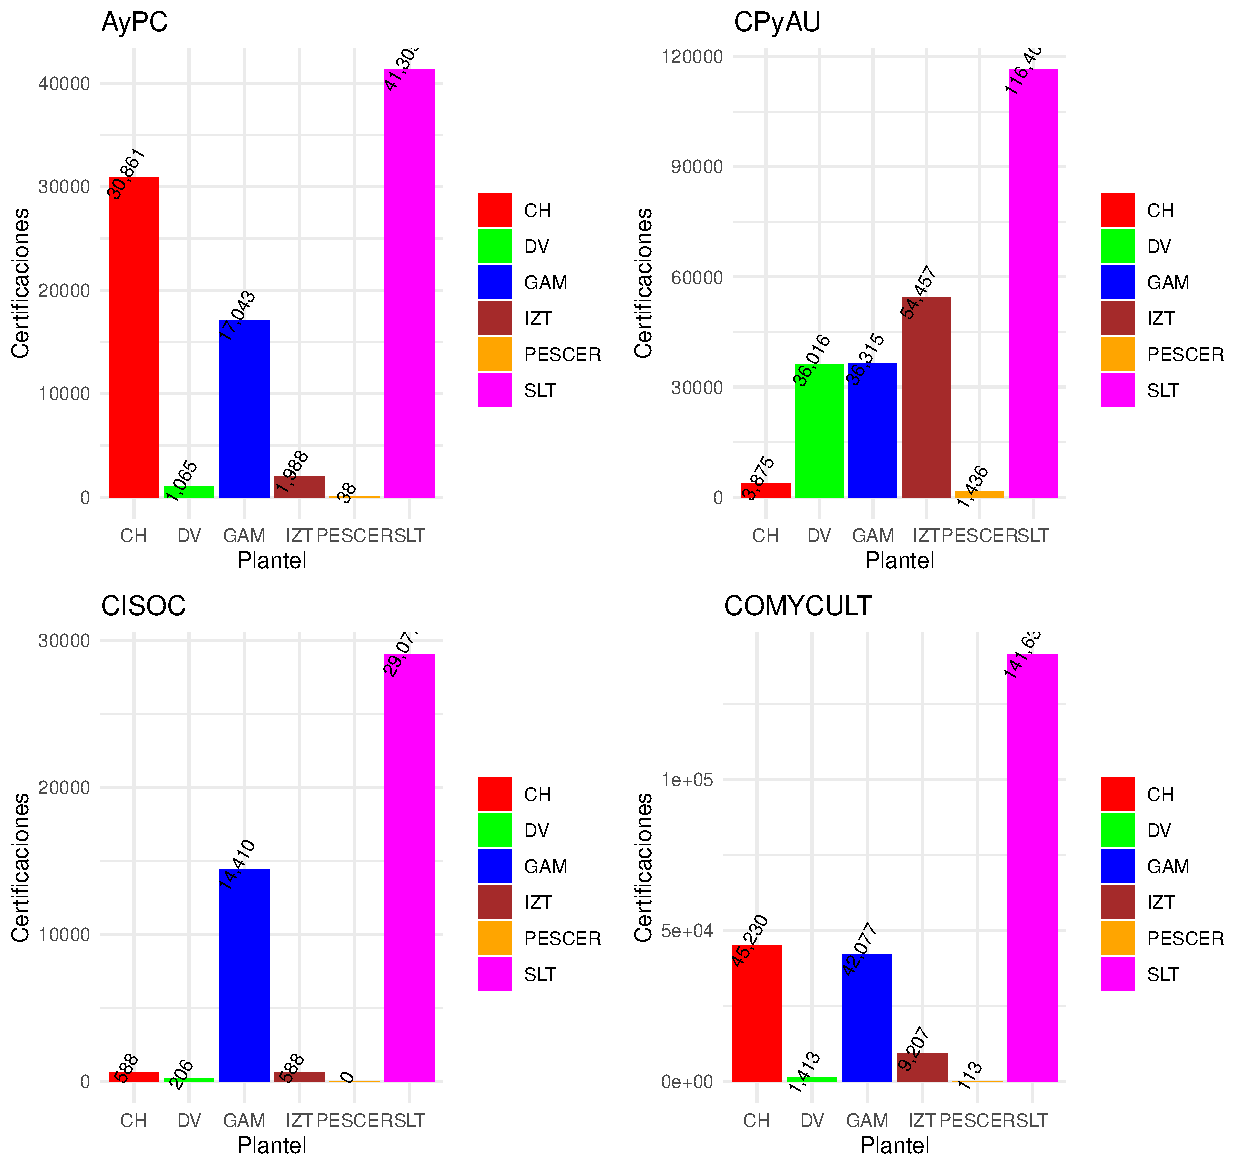
\includegraphics[width=10cm,height=5.5cm]{Imagenes/GraficasCertificacionLicenciaturas5.pdf}
\end{figure}
\end{frame}

\begin{frame}\frametitle{Certificaci\'on de licenciaturas en Planteles}
\begin{figure}[H]
\centering
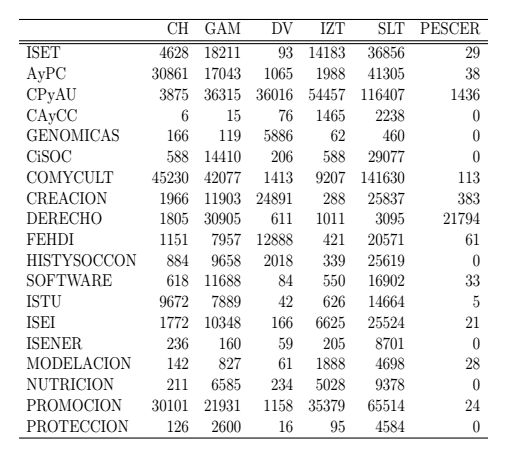
\includegraphics[width=10cm,height=5.5cm]{Tablas/CertificacionLicPlanteles.png}
\end{figure}
\end{frame}

\begin{frame}\frametitle{Certificaci\'on Favorables (licenciaturas)}
\begin{figure}[H]
\centering
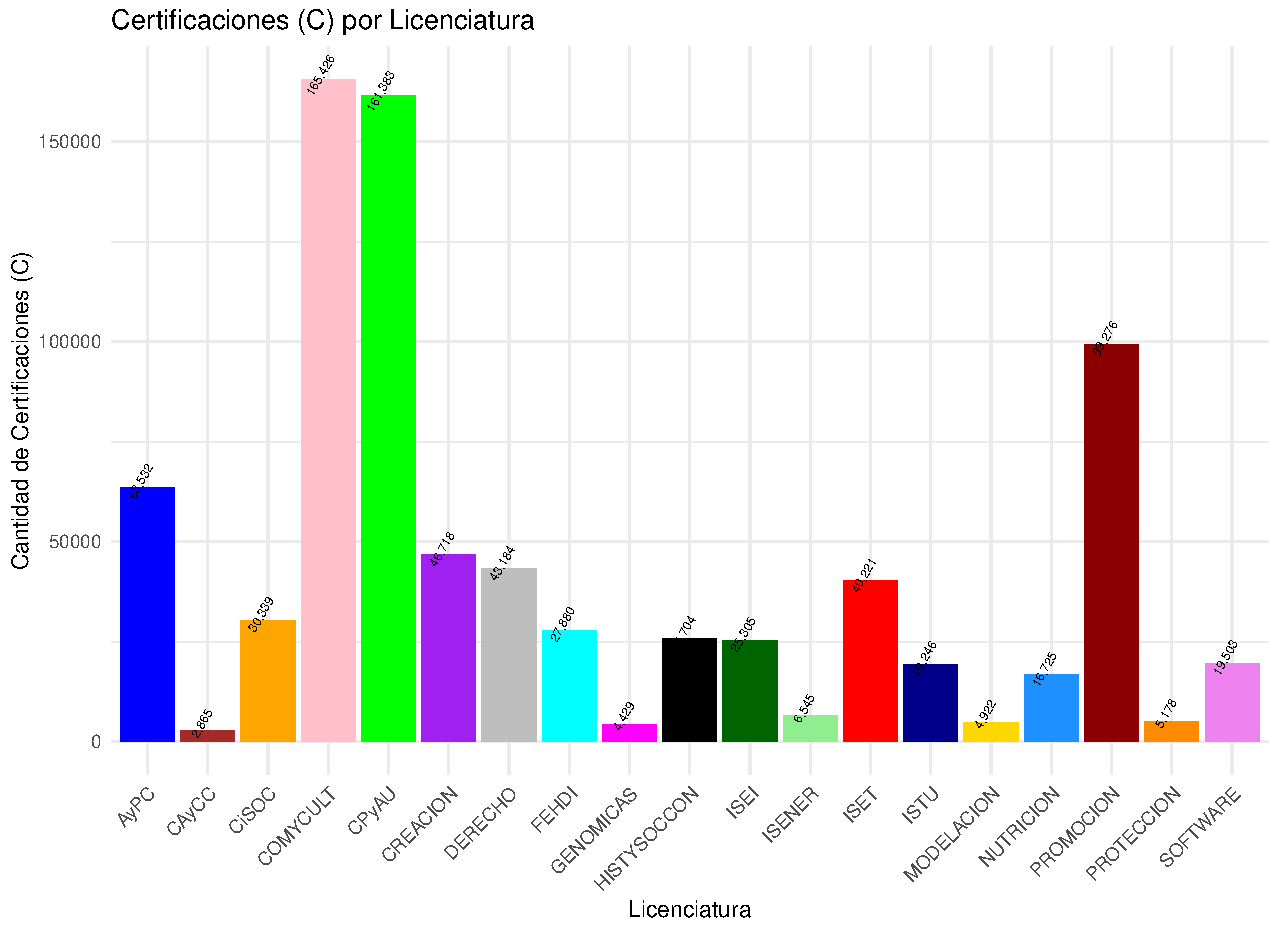
\includegraphics[width=10cm,height=5.5cm]{Imagenes/graficoCertificacionFavorableLic.pdf}
\end{figure}
\end{frame}

\begin{frame}\frametitle{Certificaci\'on No Favorables (licenciaturas)}
\begin{figure}[H]
\centering
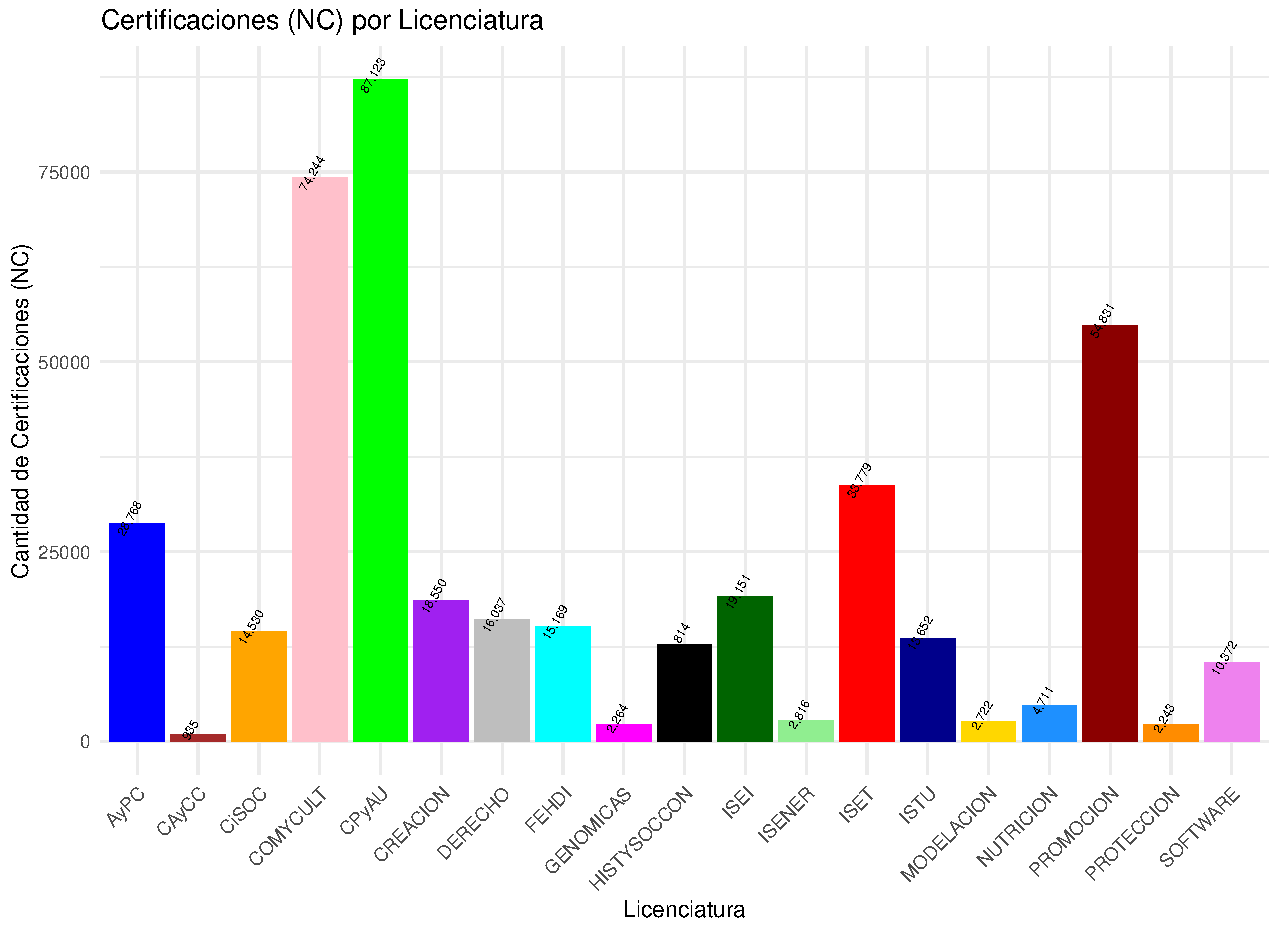
\includegraphics[width=10cm,height=5.5cm]{Imagenes/graficoCertificacionNFLicenciatura.pdf}
\end{figure}
\end{frame}

\begin{frame}\frametitle{Certificaci\'on Favorable y No Favorables en licenciaturas}
\begin{figure}[H]
\centering
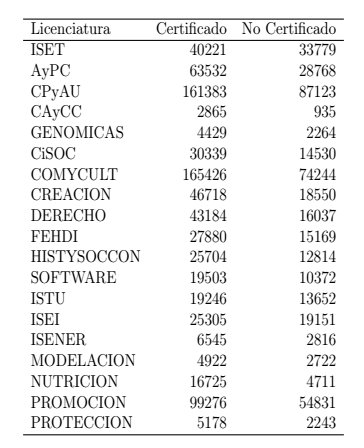
\includegraphics[width=10cm,height=5.5cm]{Tablas/CertificacionLicFnF.png}
\end{figure}
\end{frame}

\subsection{La No Certificaci\'on en la UACM}

\begin{frame}\frametitle{La No certificaci\'on en la Universidad}
\begin{figure}[H]
\centering
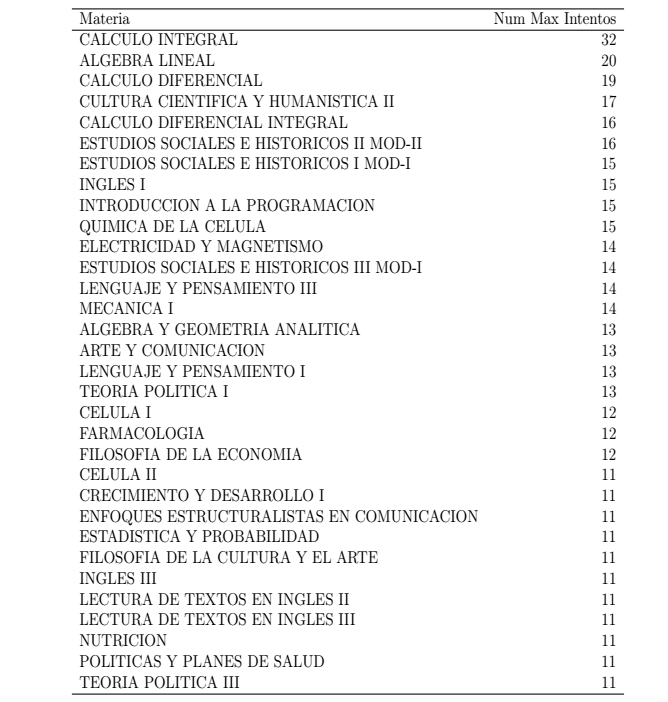
\includegraphics[width=10cm,height=5.5cm]{Tablas/MateriaMaxIntNoCert.png}
\end{figure}6
\end{frame}

\begin{frame}\frametitle{Probabilidad No Certificar}
\begin{figure}[H]
\centering
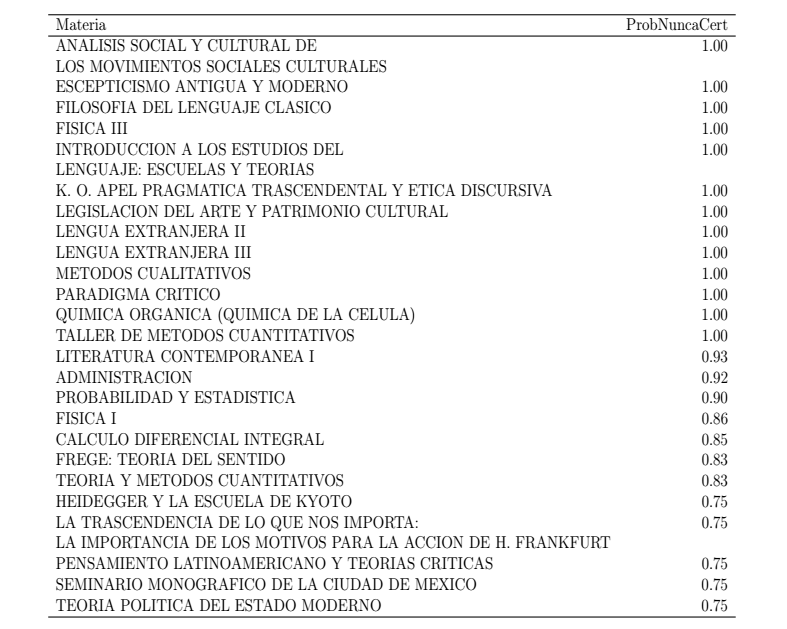
\includegraphics[width=10cm,height=5.5cm]{Tablas/MateriasNoCert.png}
\end{figure}
\end{frame}


\subsection{Certificaci\'on primer intento}

\begin{frame}\frametitle{Certificaci\'on primer intento}
\begin{figure}[H]
\centering
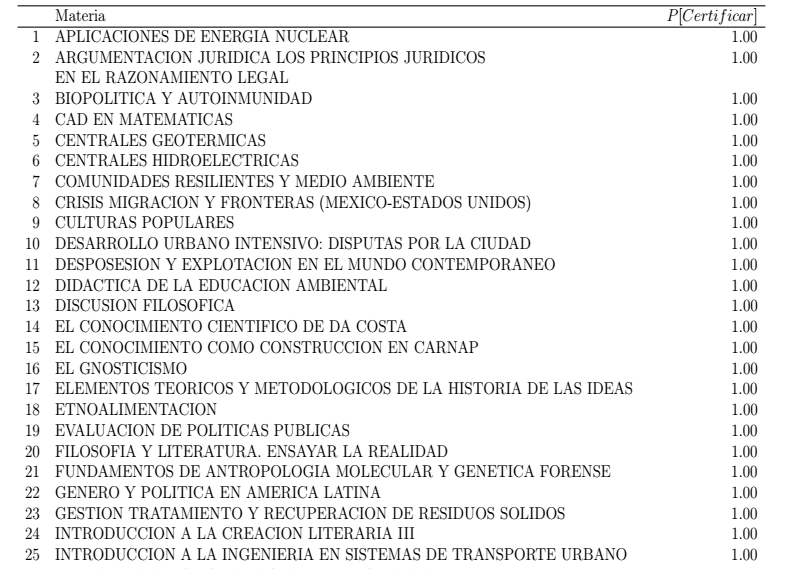
\includegraphics[width=10cm,height=5.5cm]{Tablas/MateriasCertPrimera.png}
\end{figure}
\end{frame}

\subsection{Intentos antes de certificar}

\begin{frame}\frametitle{M\'aximo Intentos antes de certificar}
\begin{figure}[H]
\centering
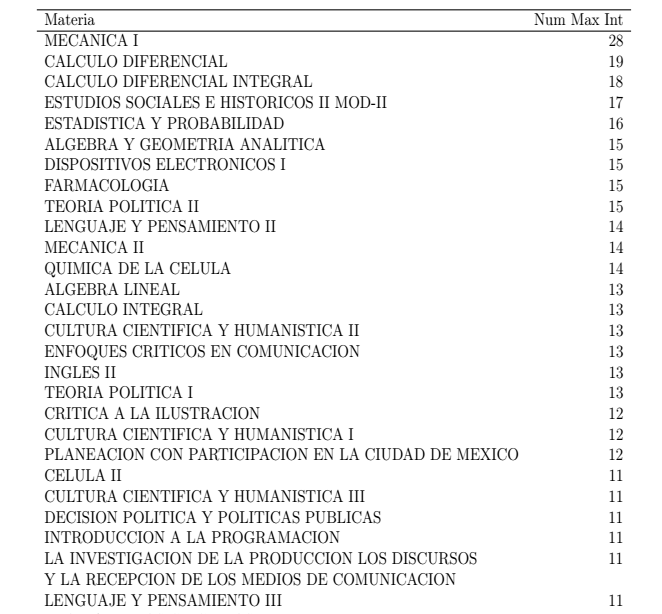
\includegraphics[width=10cm,height=5.5cm]{Tablas/MateriasMaxIntSiCert.png}
\end{figure}
\end{frame}


\begin{frame}\frametitle{Cantidad promedio de intentos antes de certificar}
\begin{figure}[H]
\centering
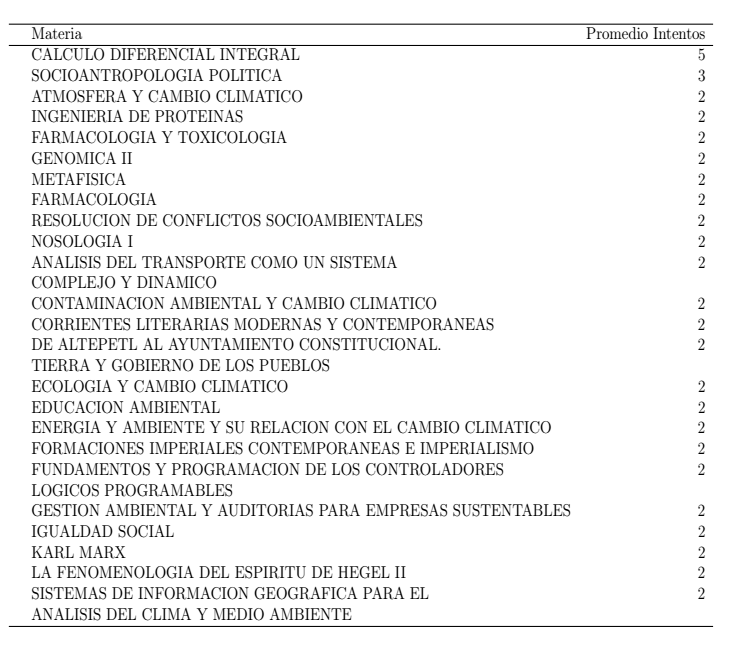
\includegraphics[width=10cm,height=5.5cm]{Tablas/MateriasPromSiCert.png}
\end{figure}
\end{frame}

\section{Trabajo futuro}


\begin{frame}
\begin{itemize}
\item Estudio de la certificaci\'on en el ciclo b\'asico y ciclo superior.

\item Estudio de la certificaci\'on en los Colegios.

\item Aplicaci\'on de modelos de clasificaci\'on y predicci\'on.

\item Inclusi\'on de los datos de registro escolar para la generalizaci\'on del estudio.

\item Vinculaci\'on con otras \'areas administrativas de la Universidad.

\item Difusi\'on y ampliaci\'on del servicio social: \textbf{UACM/SS/23027/INT}.

\item Creaci\'on del programa de Pr\'acticas Profesionales.

\item Elaboraci\'on de tesis de licenciatura.



\end{itemize}

\end{frame}




\begin{frame}

\begin{centering}
{\Huge{ Gracias!!\\
\medskip
carlos.martinez@uacm.edu.mx
}}

\end{centering}
\end{frame}




\begin{frame}

\begin{thebibliography}{20}
\bibitem{ProyectoEducativo} \textsc{UACM},
\textit{Proyecto Educativo de la UACM},
UACM, M\'exico, DF, 2004.
\bibitem{CircularCertificacion} \textsc{UACM} 
\textit{Circular para regular los procesos y registros de certificaci\'on}, M\'exico, DF, 2007.

\bibitem{Doc3} \textsc{UACM} 
\textit{En qu\'e consiste la certificaci\'on en la UACM}, M\'exico, DF, 20XX.


\end{thebibliography}
\end{frame}

\end{document}

